%======================================================================
\chapter{Cyclic Stable Matching}
%======================================================================
This chapter describes the cyclic stable matching problem as posed by Knuth. We give some sufficient conditions for a matching to be stable in this context. Then we proceed to describe a computer search procedure for deciding if all preference systems of a certain size have a cyclic stable matching or finding a counterexample should one exist. 
\section{The Problem}
\paragraph{}
In Knuth's writing on stable matching \cite{knuth1997stable} he talks about some extensions of the classical stable matching problems as discussed so far. One such avenue for generalization is increasing the number of ``genders", which is to say instead of matching pairs, we consider matching triples in tripartite graphs or more generally matching $k$-tuples in $k$-partite graphs. We will make this notion formal through the terminology of hypergraphs.
\begin{definition}
We say $G=(V,E)$ is a hypergraph if $V$ is some discrete set and $E \subseteq 2^V$ ($2^V$ denotes the set of all subsets of elements in $V$). We can think of adjacency in this case as $v \sim w$ provided there exists $e \in E$ such that $v, w \in e$. The notions of degree $d$ and edges incident upon a vertex $\delta$ extend naturally. A matching in this context is $M \subseteq E$ such that for all $m_1, m_2 \in M$, $m_1 \cap m_2 = \emptyset$. We call $G$ $k$-uniform if for all $e \in E$, $|e| = k$. We call $k$-uniform $G$ $k$-partite if there exists $V_1, \dots, V_k$ which partition $V$ and for all $e=(v_1, \dots, v_k) \in E$, $v_i \in V_i$ for $i = 1,\dots, k$. Lastly we say $k$-partite graph $G$ is balanced if $\size{V_1} = \dots = \size{V_k}$.
\end{definition}
\paragraph{}
With our description hypergraphs complete we are ready to describe a generalization of stable matching.
\begin{definition}
In an instance of cyclic $k$-gender stable matching ($kGSM$), we are given a $k$-partite hypergraph $G=(V_0 \cup \dots \cup V_{k-1}, E)$ and for each $i \in \{0,\dots,k-1\}$, each $v_i \in V_i$ is equipped with a preference order over $V_{i+1} \cap V(\delta(v_i))$ where addition of indices is taken modulo $k$ (so $V_{k-1}$ vertices have preferences over $V_0$ vertices, hence the descriptor cyclic). That is each vertex in a given gender has preferences over vertices acceptable to them in another gender. \end{definition}
\begin{definition}
We say our instance of $kGSM$, and naturally the hypergraph $G$, is complete if for all $v_0 \in V_0$, $\dots$, $v_{k-1} \in V_{k-1}$, we have $(v_0,\dots,v_{k-1}) \in E$. Hence in complete instances, which we will shorthand to $CkGSM$ instances, all possible tuples are acceptable to use in matchings.
\end{definition}
\begin{definition}
A solution to an instance of $kGSM$ is a matching $M \subseteq E$ that is stable in the sense that no blocking tuple exists. A tuple $e=(v_0,\dots, v_{k-1}) \in E$ blocks $M$ if $e\not\in M$ and for each $i \in \{0,\dots, k-1\}$, $v_{i+1} >_{v_i} M(v_i)$ where $M(v_i) \in V_{i+1}$ is the vertex satisfying that there exists an edge $m \in M$ for which $v_i, M(v_i) \in m$.
\end{definition}
\begin{note}
We may assume that instances of $kGSM$ are balanced. To see this observe that adding dummy vertices does not affect the solutions. Thus if $\size{V_i} < \size{V_j}$ we can add $\size{V_j} - \size{V_i}$ dummy vertices to $V_i$ to balance their sizes. If incomplete preferences are allowed then dummy vertices can simply have no incoming edges. If preferences are required to be complete then we may simply place dummy vertices as the least preferred vertices among the relevant preference lists and give the dummy vertices arbitrary orders over ``real" vertices they face. We say that an instance of $kGSM$ is of size $n$ if it is balanced with each $V_i$ having size $n$.
\end{note}
\paragraph{}
We will focus on instances where $k=3$ to simplify things somewhat. Knuth asked if instances of $3GSM$ always have stable solutions. To this day this question is unresolved for complete instances. Some, but not many, results are known and we will present them in the next section.
\begin{conjecture}\label{conj:unstab}
(Knuth) For all sizes $n$, instances of $3GSM$ of size $n$ have a stable matching.
\end{conjecture} 
\section{Known Results}
\paragraph{}
First we will present a counterexample that demonstrates that when instances are not complete there need not always be a stable matching solution. This example is due to Biro et al. \cite{biro2010three} and shows that when there are incomplete preferences there is a hypergraph with each $V_i$ having size $6$ and preference lists that admit no stable matching.
\begin{note}\label{ex:R6}
For our counterexample consider the tripartite hypergraph $R6 = (A \cup B \cup C, E)$ where $$A = \{a_0, a_1,a_2,a_0', a_1',a_2'\},\ B = \{b_0, b_1,b_2,b_0',b_1',b_2'\},\ \text{and}\ C = \{c_0,c_1,c_2,c_0',c_1',c_2'\}.$$ Below we present the preference orders of each vertex, where vertices omitted from a list are deemed unacceptable and cannot form edges with the given vertex whose list is under consideration:
\begin{align*}
a_0 &: b_0 > b_0' &b_0: c_0 > c_0' &\ &c_0:a_1 > a_1'\\
a_1 &: b_1 > b_1' &b_1: c_1 > c_1' &\ &c_1:a_2 > a_2'\\
a_2 &: b_2 > b_2' &b_2: c_2 > c_2' &\ &c_2: a_0> a_0'\\
a_0' &: b_2 &b_0': c_2 &\ &c_0':a_0 \\
a_1'&: b_0 &b_1': c_0 &\ &c_1':a_1\\
a_2' &:b_1 &b_2': c_1 &\ & c_1':a_2.
\end{align*}
We will adopt the notation of the original authors calling the agents $\{a_i, b_i, c_i: 1 \leq i \leq 3 \}$ the inner agents and $\{a_i',b_i',c_i': 1\leq i \leq 3\}$ the outer agents.
\end{note}.
\begin{lemma}
The problem instance of $3GSM$ described in note \ref{ex:R6} has no stable matching.
\end{lemma}
\begin{proof}
Let $M$ be a matching in $R6$. We observe that the possible triples in $M$ have very particular forms. Let $m \in M$ be a triple. Suppose that inner vertex $a_i$ is in $m$. Then by $a_i$'s preferences either $b_i \in m$ or $b_i' \in m$. If $b_i \in m$ then as $a_i$ is not acceptable to $c_i$, the triple $m$ is of the form $a_ib_ic_i'$. If $b_i' \in m$ then $c_{i-1} \in m$ (recall index addition and subtraction is done modulo $3$) and hence the triple $m$ is of the form $a_i b_i'c_{i-1}$. Otherwise if outer vertex $a_i' \in m$ then the triple $m$ is of the form $a_i'b_{i-1}c_{i-1}$. That is the only triples in $M$ are those of the form
$$a_ib_ic_i' \quad\text{or}\quad a_ib_i'c_{i-1} \quad\text{or}\quad a_i'b_{i-1}c_{i-1}.$$
Then triples in $M$ contain exactly two inner agents and one outer agent each. Since each agent can only be matched at most once, and inner agents are matched in pairs then $M$ matches an even number of inner agents. But there are an odd number of inner agents ($9$ to be precise). Hence at least one inner agent is unmatched in $M$. By the symmetry of $R6$ we may assume without loss of generality that this inner agent is $a_i$. Consider the triple $T=(a_i, b_{i}', c_{i-1})$. If $c_{i-1}$ is matched in $M$ then, as $a_i$ is unmatched, $M(c_{i-1}) = a_i'$. Hence $a_i >_{c_{i-1}} M(c_{i-1})$. Again since $a_i$ is unmatched, $b_{i}'$ is unmatched and thus prefers $T$ to $M$. Hence the triple $T$ blocks $M$, and since $M$ was an arbitrary matching no matching of $R6$ is stable.
\end{proof}
\paragraph{}
Since we have a counterexample to stability in the case where incomplete preferences are allowed this motivates us to restrict the problem to the situation where problem instances are complete. It is in this setting that we will work going forward. As of yet we are not aware of any counterexample instance that has no stable matching for complete $3GSM$ ($C3GSM$), nor of any proof that all instances admit a stable matching. Thus we consider a modified conjecture for $C3GSM$ instances as follows.
\begin{conjecture}\label{conj:stab}
(Knuth) For all sizes $n$, instances of $C3GSM$ of size $n$ have a stable matching.
\end{conjecture} 
\paragraph{}
One natural angle towards a proof would be to attempt to extend the Deferred-Acceptance algorithm of Gale and Shapley to $C3GSM$. Farczadi et al. provide some insight into the feasibility of this route in \cite{farczadi2014stable}. Here they claim a certain step in the natural approach to extending Deferred-Acceptance is $NP$-complete. For readers without a complexity theory background this result gives strong evidence that there is no polynomial time algorithm for the concrete approach to extending Deferred-Acceptance examined in \cite{farczadi2014stable}.
\begin{definition}
Let $G = (A\cup B \cup C, E)$ be a hypergraph underlying an instance of $C3GSM$. Let $M'$ be a matching of $A$ to $B$. We say that a matching $M$ in $G$ is an extension of $M'$ if for all $a \in V(M') \cap A$, $M'(a) = b$ implies $M(a) = b$.
\end{definition}
\begin{theorem}
(Farczadi et al.): Consider an instance of $C3GSM$ with hypergraph $G=(A\cup B\cup C, E)$. Fix a perfect matching of $A$ to $B$. The problem of deciding if this matching can be extended to a stable matching of $G$ is $NP$-complete.
\end{theorem}
\paragraph{}
So in lieu of algorithmic insight into the problem, researchers have presented ad-hoc methods to demonstrate when instances of $C3GSM$ are stable for fixed sizes $n$. It has been shown by Eriksson et al. \cite{eriksson2006three} that complete instances of size $n \leq 4$ always have a stable matching. First observe that cases of size $n \leq 2$ are not interesting as blocking triples are impossible since a blocking triple must draw each of its vertices from a distinct triple in the matching (no vertices in instances of $C3GSM$ are unmatched in a stable matching, as there would be at least three and they prefer to be together than unmatched). The case for $n=3$ is straightforward and can even be checked by hand. Eriksson et al. have shown something stronger for the $n=3$ case: that they can actually fix the quality of match any arbitrary vertex receives in a stable matching. We will present below some notation to ease exposition then give their proof.
\begin{definition}
Let $G=(A\cup B \cup C, E)$ be the hypergraph for an instance of $C3GSM$. We will define the following functions for $A$ but we will use analogous versions for $B$ and $C$ throughout. Let $a \in A$. Let $s \in \{1,\dots,n\}$. If $s=1$ define $f(G,a,s) = b$ provided for all $b' \in B$, $b \geq_a b'$. If $s>1$ define $f(G,a,s) = b$ provided $$f(G[V(G) \backslash \{f(G,a,t): t\in\{1,\dots,s-1\}], a, 1) = b.$$ Intuitively $f(G,a,s)$ is $a$'s $s$-th choice among vertices in $B$ where $G = (A\cup B \cup C, E)$.
\end{definition}
\begin{definition}
Let $G = (A \cup B \cup C, E)$ be the hypergraph for an instance of $C3GSM$. We say $G$ has an $i,j,k$ triple if there exist $a \in A$, $b\in B$, and $c \in C$ such that $f(G,a,i) = b$, $f(G,b,j) = c$, and $f(G,c,k) = a$. Of particular interest are $1,1,1$ triples. If a matching contains a $1,1,1$ triple then none of the vertices in the triple will participate in any blocking triple against the matching.
\end{definition}
\begin{lemma}\label{lemma:n3}
(Eriksson et al.) \cite{eriksson2006three}: Let $G=(A\cup B \cup C, E)$ be the hypergraph for an instance of $C3GSM$ of size $3$. Let $a \in A$. Then $G$ has a stable matching $M$ where either $M(a)= f(G,a,1)$ or, $M(a) = f(G,a,2)$ and $M(b) = f(G,b,1)$ where $b = f(G,a,1)$.
\end{lemma}
\begin{proof} First consider the case where $G$ has a $1,1,1$ triple $(a',b',c')$. Construct the matching $M$ as follows. Add $a'b'c'$ to $M$. Now $a',b',c'$ will not participate in any blocking triples against $M$. Hence there are only $6$ vertices remaining, so regardless of how we choose the next two triples for $M$ the resulting matching will be stable. If $a = a'$ then we are done, so we may assume $a\neq a'$. If $b = b'$ then complete $M$ arbitrarily as long as $M(a) = f(G,a,2)$. Otherwise, $b\neq b'$ and we may complete $M$ arbitarily ensuring $M(a) = b$.
\paragraph{} Now consider the case where $G$ has no $1,1,1$ triple. Let $c = f(G,b,1)$. Since there is no $1,1,1$ triple, $a \neq f(G,c,1)$. Let $a' = f(G,c,1)$. Again since there is no $1,1,1$ triple $b \neq f(G,a',1)$. Let $b' = f(G,a',1)$. Similarly $c \neq f(G,b',1)$ and let $c' = f(G,b',1)$. Let $a'', b'', c''$ be the remaining vertices in $A,B,C$ respectively. Form the matching $M = \{abc,a'b'c',a''b''c''\}$. We claim $M$ is stable. Since $a$ and $a'$ were matched to their first choices they will not participate in any blocking triple. Hence $a''$ is the only vertex in $A$ willing to participate in a blocking triple. But $a'$ is only unmatched to $b$ and $b'$, both of which are matched to their first choices and hence are unwilling to participate in any blocking triple. Thus there are no blocking triples against $M$ and hence $M$ is stable. Further since $M(a) = b$ we are done. 
\end{proof}
\paragraph{}
Using lemma \ref{lemma:n3} Eriksson et al. show the following theorem. We omit the proof as, by the authors own admission, it is a technical case analysis.
\begin{theorem}(Eriksson et al.) \label{theorem:n4} \cite{eriksson2006three}: The conjecture \ref{conj:stab} holds for $n\leq 4$.
\end{theorem}
\section{Our Contributions}
\paragraph{}
In this section we will describe some work done towards resolving if $C3GSM$ instances always have solutions for higher sizes $n\geq 5$. We present first some sufficient conditions for problem instances to have stable matchings. Next we study the symmetry of problem instances and describe when problem instances are equivalent with respect to having a stable matching. All this work is building towards a proposal for a computer search procedure to decide if all instances of $C3GSM$ for a given size $n$ have a stable matching, or present a counterexample if they do not.
\subsection{Sufficient Conditions}\label{subsec:sufficient}
\begin{definition}
Let $G$ be the hypergraph for an instance of $C3GSM$, and let $M$ be a matching in $G$. We denote by $\cB(G,M)$ the set of blocking triples in $G$ against $M$. Formally $\cB(G,M) = \{abc \in E(G): b>_a M(a), c>_b M(b), a>_c M(c)\}$. We denote the set of discontent vertices, those that participate in blocking triples, as $\cD(G,M) = V(\cB(G,M))$.
\end{definition}
\begin{note}
If we let $S \subseteq V(G)$ and denote by $G[S]$ the hypergraph $G$ restricted to vertices in $S$ and edges between vertices in $S$ ($G[S]$ denotes the subgraph induced by $S$) then we may use $\cB(G[S],M)$ to describe the blocking triples of $G$ among vertices in $S$. In particular if we wish to study blocking triples present among agents matched in $M$ we study the set $\cB(G[V(M)], M)$.
\end{note}
\begin{note}
We mention a few things here that are immediately obvious from the definition of $\cD$. Let $G=(A\cup B \cup C, E)$ be a hypergraph underlying an instance of $C3GSM$. Let $M$ be a matching in $G$. Then we have:
\begin{itemize}
\item If $M'$ is matching such that $M \subseteq M'$ then $\cD(G,M') \subseteq \cD(G,M)$.
\item $M$ is a stable matching in $G$ if and only if $\cD(G, M) = \emptyset$.
\item If $v \in \cD(G,M)$ then there exists $w >_v M(v)$ such that $w \in \cD(G,M)$.
\end{itemize}
\end{note}
\paragraph{}
Sometimes we want to talk about the vertices that some given vertices can form blocking triples with. The following definition captures this idea.
\begin{definition}
Let $G$ be the hypergraph underlying an instance of $C3GSM$. Let $W \subseteq V(G)$. We define $\cD(G,M, W) = \{v \in \cD(G,M): \exists w\in W: v>_w M(w) \}$.
\end{definition}
\paragraph{}
The following lemma underlies a common approach to finding stable matchings. In it we demonstrate how a partial matching can be used to construct a complete stable matching.
\begin{lemma}\label{lemma:inductive}
Let $G=(A\cup B \cup C, E)$ be a hypergraph underlying an instance of $C3GSM$ of size $n$, where $n-1$ is the best known size that satisfies conjecture \ref{conj:stab}. Suppose there exists a non-empty matching $M$ in $G$ such that $V(M) \cap \cD(G,M) = \emptyset$. Then $G$ has a stable matching.
\end{lemma}
\begin{proof}
Let $G' = G[V(G)\backslash V(M)]$ be the subgraph of $G$ induced by vertices unmatched in $M$.  Consider the instance of $C3GSM$ with underlying hypergraph $G'$ and preference orders induced by $G$. Since $M \neq \emptyset$ the size of this new instance is at most $n-1$. Hence by conjecture \ref{conj:stab} there exists a stable matching $M'$ in $G'$. Let $S = M \cup M'$. Then $S$ is a perfect matching in $G$. We claim that $S$ is stable. Indeed since $M \subseteq S$ and $V(M) \cap \cD(G,M) = \emptyset$ we have that $V(M) \cap \cD(G,S) = \emptyset$. So $\cD(G,S) \subseteq V(M')$. Since $V(M') = V(G')$ if $\cD(G,S)$ is non-empty then $\cD(G', M')$ is non-empty, contradicting that $M'$ is a stable matching in $G'$. Thus $\cD(G,S) = \emptyset$ and therefore $S$ is a stable matching in $G$.
\end{proof}

\paragraph{}
The following lemma gives a condition that is faster to check than the previous lemma, but still covers some common cases.

\begin{lemma}\label{lemma:partialstab}
Let $G = (A\cup B \cup C, E)$ be the hypergraph for an instance of $C3GSM$ of size $n$ where $n-1$ is the best known size that  satisfies conjecture \ref{conj:stab}. Suppose that $G$ has a non-empty matching $M$ for which $\cB(G[V(M)],M) = \emptyset$. If $$\{w \in V(G): \exists v \in V(M), w >_v M(v)\} \subseteq V(M)$$ then $G$ has a stable matching.
\end{lemma}
\begin{proof}
Let $a \in V(M)$. Suppose there exists $abc \in \cB(G,M)$. Since $b >_a M(a)$ and $a \in V(M)$, we have that $b \in V(M)$. Similarly since $c >_b M(b)$ we have that $c \in V(M)$. Further since $a >_c M(a)$ we have that $abc \in \cB(G[V(M)],M)$, contradicting that $\cB(G[V(M)],M) = \emptyset$. Hence for all $e \in \cB(G,M)$, $a \not\in e$. Thus $a\not \in \cD(G,M)$ and therefore $V(M) \cap \cD(G,M) = \emptyset$. So by lemma \ref{lemma:inductive} $G$ has a stable matching.
\end{proof}
\paragraph{Example}
Consider the following instance of $C3GSM$ and focus on the bolded preferences:
\begin{align*}
a_0 &: \boldsymbol{b_1} > \boldsymbol{b_0} > b_2 > b_3 > b_4    &b_0: \boldsymbol{c_1} > \boldsymbol{c_0}  > c_2 > c_3 > c_4   &\ &c_0:\boldsymbol{a_1} > \boldsymbol{a_0} > a_2 > a_3 > a_4\\
a_1 &: \boldsymbol{b_0} > \boldsymbol{b_1} > b_4 > b_2 > b_3    &b_1: \boldsymbol{c_0} > \boldsymbol{c_1}  > c_3 > c_4 > c_2  &\ &c_1:\boldsymbol{a_0} > \boldsymbol{a_1} > a_2 > a_3 > a_4\\
a_2 &: b_2 > b_1 > b_0 > b_3 > b_4    &b_2: c_2 > c_1 > c_3 > c_4 > c_0    &\ &c_2: a_0 > a_2 > a_3 > a_4 > a_1\\
a_3 &: b_1 > b_0 > b_3 > b_4 > b_3    &b_0': c_3 > c_4 > c_2 > c_1 > c_0   &\ &c_3:a_1 > a_0 > a_3 > a_2 > a_4 \\
a_4 &: b_0 > b_2 > b_3 > b_4 > b_1    &b_1': c_0 > c_1 > c_2 > c_3 > c_4   &\ &c_4:a_4 > a_3 > a_2 > a_1 > a_0\\
\end{align*}
Matching $M = \{a_0b_0c_0, a_1b_1c_1\}$ satisfies lemma \ref{lemma:partialstab}. Therefore $M$ and any stable matching of $a_2,a_3,a_4,b_2,b_3,b_4,c_2,c_3,c_4$ together form a stable matching in this problem instance.
\begin{corollary}\label{cor:1cycle}
Let $G$ be the hypergraph for an instance of $C3GSM$ and $n$ be as in lemma \ref{lemma:partialstab}. If there exists $a,b,c \in V(G)$ such that $b = f(G,a,1)$, $c = f(G,b,1)$, and $a = f(G,c,1)$ (a $1,1,1$ triple) then $G$ has a stable matching.
\end{corollary}
\begin{proof}
Invoke lemma \ref{lemma:partialstab} with $M = \{(a,b,c)\}$.
\end{proof}
\begin{corollary}
Let $G=(A\cup B \cup C, E)$ be the hypergraph for an instance of $C3GSM$ with $n$ as in lemma \ref{lemma:partialstab}. If one of $A,B,C$, say without loss $A$, is such that there exists $b \in B$, for all $a \in A$, $f(G,a,1) = b$ then $G$ has a stable matching.
\end{corollary}
\begin{proof}
Let $a_1, \dots, a_n \in A$. Let $c = f(G,b,1)$. Then there exists some $a_k$ such that $a_k = f(G,c,1)$. Since $a_k \in A$ we may invoke corollary \ref{cor:1cycle} with $(a_k, b, c)$ to complete the proof.
\end{proof}

\paragraph{}
The follow lemmas study situations where we nearly have a matching which satisfies $\cD(G,M) = \emptyset$ except some part, without loss $A$, has vertices which form some limited blocking triples. The first lemma looks to build a matching containing $M$ and using lemma \ref{lemma:inductive} to find a stable matching. The second lemma shows that if the matching $M$ is large enough if implies the existence of a stable matching directly.

\begin{lemma} \label{lemma:partial-match}Let $G=(A\cup B \cup C, E)$ be the hypergraph underlying an instance of $C3GSM$ of size $n$ where $n-1$ is the best known size satisfying conjecture \ref{conj:stab}. Let $M$ be a matching in $G$. Suppose that
$$ V(M) \cap (B \cup C) \cap \cD(G,M) = \emptyset$$
and that there exists $b \in B\backslash V(M)$ satisfying
$$ \cD(G, M, V(M) \cap A)  = \{b\}$$
and for all $a \in A \backslash V(M)$, $f(G[V(G)\backslash V(M)], a, 1) = b$. Then $G$ has a stable matching.
\end{lemma}
\begin{figure}[h]
\centering
\begin{tikzpicture}
\Vertex[x=0,y=6,L=$a_0$]{a0}
\Vertex[x=3,y=6,L=$b_0$] {b0}
\Vertex[x=6,y=6,L=$c_0$]{c0}

\Vertex[x=0,y=4,L=$a_1$]{a1}
\Vertex[x=3,y=4,L=$b_1$] {b1}
\Vertex[x=6,y=4,L=$c_1$]{c1}



\Vertex[x=0,y=2,L=$a_2$]{a2}
\Vertex[x=3,y=2,L=$b_2$] {b2}
\Vertex[x=6,y=2,L=$c_2$]{c2}

\Vertex[x=0,y=0,L=$a_3$]{a3}
\Vertex[x=3,y=0,L=$b_3$] {b3}
\Vertex[x=6,y=0,L=$c_3$]{c3}

\Vertex[x=0,y=-2,L=$a_4$]{a4}
\Vertex[x=3,y=-2,L=$b_4$] {b4}
\Vertex[x=6,y=-2,L=$c_4$]{c4}

\tikzstyle{EdgeStyle}=[post]

\Edge[label=$\{b_2\}$](a0)(b0)
\Edge[label=$\emptyset$](b0)(c0)

\Edge[label=$\{b_2\}$](a1)(b1)
\Edge[label=$\emptyset$](b1)(c1)

\tikzstyle{EdgeStyle}=[post,bend right]
\Edge[label=$\emptyset$](c0)(a0)
\Edge[label=$\emptyset$](c1)(a1)

\tikzstyle{EdgeStyle}=[dashed,post]
\Edge[](a2)(b2)
\Edge[](a3)(b2)
\Edge[](a4)(b2)
\Edge[](b2)(c2)
\tikzstyle{EdgeStyle}=[dashed,post,bend left]

\Edge[](c2)(a2)
\end{tikzpicture}
\caption{Visualizing lemma \ref{lemma:partial-match}}
\small
\begin{flushleft}
Solid arcs indicate matching $M$, and are labelled with $\cD(G,M,\{t\})$ where $t$ is the tail vertex of the arc. Dashed arcs indicate first choice of tail vertex outside $V(M)$.
\end{flushleft}
\end{figure}

\begin{proof}
Let $G' = G[V(G)\backslash V(M)]$ be the subgraph of $G$ induced by vertices unmatched in $M$. Let $c = f(G',b,1)$ and $a = f(G',c,1)$. By our hypothesis, $b = f(G',a,1)$. Let $T = \{abc\}$. Consider the matching $M' = M \cup T$. We will show that $V(M') \cap \cD(G, M') = \emptyset$ to invoke lemma \ref{lemma:inductive} to complete the proof.
\paragraph{}
Let $v \in V(M')$. First consider the case where $v \in V(M) \cap ( B \cup C)$. Since $v \not\in \cD(G,M)$ and $M \subseteq M'$, we have that $v \not\in \cD(G,M')$. Second consider the case where $v \in \{a,b\}$. If $w >_v M'(v)=T(v)$ then $w \in V(M) \cap (B \cup C)$ by our construction of $T$. Since such $ w\not\in \cD(G,M')$ we have $v \not\in \cD(G,M')$. Third consider the case where $v \in V(M) \cap A$. By our hypothesis if $w >_v M'(v) = M(v)$ then $w = b$. Since $b \not\in \cD(G,M')$ we have $v \not\in \cD(G,M')$. Finally consider the case where $v = c$. Since $v \in T$, by our construction of $T$, if $w >_v M'(v)$ then $w \in V(M) \cap A$. Since such $w \not\in \cD(G,M')$ we have $v \not\in \cD(G,M')$. Therefore $V(M') \cap \cD(G,M') = \emptyset$, and since $T \subseteq M'$,  we have $M' \neq \emptyset$ so we may apply lemma \ref{lemma:inductive} to conclude that $G$ has a stable matching.
\end{proof}
\begin{lemma}
Let $G=(A\cup B \cup C, E)$ be the hypergraph underlying an instance of $C3GSM$ of size $n$. Let $M$ be a matching in $G$ such that $|M| \geq n-3$. Suppose that 
$$V(M) \cap C \cap \cD(G,M) = \emptyset$$
and there exists $b \in B \backslash V(M)$ satisfying
$$\cD(G,M,V(M) \cap A) = \{b\}$$
and for all $a \in A \backslash V(M)$, $f(G[V(G)\backslash V(M)], a, 1) = b$. Suppose also that there exists $c \in C \backslash V(M)$ satisfying
$$\cD(G,M,V(M) \cap B ) = \{c\}.$$ 
Then $G$ has a stable matching.
\end{lemma}
\begin{proof}
Let $G' = G[V(G)\backslash V(M)]$ be the subgraph of $G$ induced by vertices unmatched in $M$. Let $c' = f(G',b,1)$ be the first choice of $b$ unmatched in $M$. We consider two cases: when $c' = c$ and when $c' \neq c$.

\paragraph{} First consider when $c' = c$.  Let $a' = f(G',c', 1)$ be the first choice of $c'$ unmatched in $M$. Let $T = \{a'bc\}$. Let $M' = M \cup T$. We will show $V(M') \cap \cD(G,M') =\emptyset$. Let $v \in V(M')$. We give the following case analysis on $v$:
\begin{itemize} 
\item If $v \in V(M) \cap C$ then $v \not\in \cD(G,M')$ since $M \subseteq M'$.
\item If $v = b$ then $w >_v M'(v) = c$ implies $w \in V(M') \cap C$ by our construction of $T$. Thus $w \not\in \cD(G,M')$ and so $v \not\in \cD(G,M')$.
\item If $v \in V(M) \cap A$ then $w >_v M'(v) = M(v)$ implies $w = b$ by our hypothesis. Since $b \not\in \cD(G,M')$ we thus have $v \not\in \cD(G,M')$. 
\item If $v = c$ then $w>_v M'(v) = T(v)$ implies $w \in V(M') \cap A$ and thus $w \not\in \cD(G,M')$, so $v\not\in \cD(G,M')$.
\item If $v \in V(M) \cap B$ then $w>_v M'(v)=M(v)$ implies $w = c$ and thus $w \not\in \cD(G,M')$, so $v \not\in \cD(G,M')$.
\item If $v = a'$ then $w >_v M'(v) = T(v)$ implies that $w \in V(M') \cap B$ by our construction of $T$. Thus $w\not\in \cD(G,M')$ and so $v\not\in \cD(G,M')$. 
\end{itemize}
Therefore $V(M') \cap \cD(G,M') = \emptyset$. Let $S$ be an arbitrary perfect matching in $G$ such that $M' \subseteq S$. Since $|M'| \geq n-2$, $|S\backslash M'| \leq 2$. Since $V(M') \cap \cD(G,M')$ any blocking triple against $S$ must use one vertex from each of three edges in $S\backslash M'$, but since $|S\backslash M'| \leq 2$ this implies it is impossible to form a blocking triple against $S$.
\paragraph{}
Now consider the case when $c' \neq c$. Let $a = f(G',c,1)$. Let $a' = f(G'[V(G')\backslash a], c',1)$ be the first choice of $c'$ among vertices unmatched in $M$ and excluding $c$'s first choice, $a$. Let $b' = f(G'[V(G')\backslash b], a, 1)$. Let $T = \{ab'c\}$ and $T' = \{a'bc'\}$. Form the matching $M' = M \cup T \cup T'$. Again we study $V(M') \cap \cD(G,M')$. Let $v \in V(M')$. In the same manner as the analysis for the previous case, we observe $V(M) \cap C \cap \cD(G,M') = \emptyset$, $b \not \in \cD(G,M')$, $V(M) \cap C \cap \cD(G,M') = \emptyset $, $c\not\in \cD(G,M')$, and $V(M) \cap B \cap \cD(G,M') = \emptyset$, and $a' \not\in \cD(G,M')$. So it remains to consider $v \in \{a, b', c'\}$:
\begin{itemize}
\item If $v = a$ then $w>_a M'(a) = b'$ implies that $w \in V(M) \cap B$ or $w = b$. In either case $w$ is not in $\cD(G,M')$ and thus $v \not\in \cD(G,M')$.
\item If $v = c'$ then $w>_{c'} M'(c') = a$ implies that $w \in V(M) \cap A$ or $w = a$. In either case $w$ is not in $\cD(G,M')$ and thus $v \not\in \cD(G,M')$.
\end{itemize}
Now we did not explicitly choose the partner of $b'$ based on her preference, so we cannot perform the above line of reasoning to conclude that $b' \not\in \cD(G,M')$. Therefore $V(M') \cap \cD(G,M') \subseteq \{b'\}$. Let $S$ be an arbitrary perfect matching of $G$ such that $M' \subseteq S$. Since $|M'| \geq n-1$ and $V(M') \cap \cD(G,M')$ there is exactly  one triple $e \in S \backslash M'$, and the vertex $b'$ from which any blocking triple against $S$ in $G$ could draw its vertices. This is insufficient to form a blocking triple and thus $S$ is a stable matching in $G$.
\end{proof}

\begin{lemma}\label{lemma:fixing}
Let $G = (A\cup B \cup C, E)$ be the hypergraph underlying an instance of $C3GSM$ of size $n$. Let $M$ be a matching in $G$ with $\size{M} = n-2$. Suppose there exists $a \in A \cap V(M)$ such that $$V(M) \cap \cD(G,M) = \{a\}.$$ If $f(G, a, $n$)$ is not in $V(M)$ then $G$ has a stable matching.
\end{lemma}
\begin{figure}[h]
\centering
\begin{tikzpicture}
\Vertex[x=0,y=6,L=$a_0$]{a0}
\Vertex[x=3,y=6,L=$b_0$] {b0}
\Vertex[x=6,y=6,L=$c_0$]{c0}

\Vertex[x=0,y=4,L=$a_1$]{a1}
\Vertex[x=3,y=4,L=$b_1$] {b1}
\Vertex[x=6,y=4,L=$c_1$]{c1}



\Vertex[x=0,y=2,L=$a_2$]{a2}
\Vertex[x=3,y=2,L=$b_2$] {b2}
\Vertex[x=6,y=2,L=$c_2$]{c2}

\Vertex[x=0,y=0,L=$a_3$]{a3}
\Vertex[x=3,y=0,L=$b_3$] {b3}
\Vertex[x=6,y=0,L=$c_3$]{c3}

\Vertex[x=0,y=-2,L=$a_4$]{a4}
\Vertex[x=3,y=-2,L=$b_4$] {b4}
\Vertex[x=6,y=-2,L=$c_4$]{c4}

\tikzstyle{EdgeStyle}=[post]

\Edge[label=$\emptyset$](a0)(b0)
\Edge[label=$\emptyset$](b0)(c0)

\Edge[label=$\emptyset$](a1)(b1)
\Edge[label=$\emptyset$](b1)(c1)

\Edge[label=$\{b_3\}$](a2)(b2)
\Edge[label=$\emptyset$](b2)(c2)

\tikzstyle{EdgeStyle}=[post,bend right]
\Edge[label=$\emptyset$](c0)(a0)
\Edge[label=$\emptyset$](c1)(a1)
\Edge[label=$\emptyset$](c2)(a2)

\end{tikzpicture}
\caption{Visualizing lemma \ref{lemma:fixing}}
\small
\begin{flushleft}
Solid arcs indicate matching $M$, and are labelled with $\cD(G,M,\{t\})$ where $t$ is the tail vertex of the arc. In this figure $b_4$ is the last choice of $a_2$.
\end{flushleft}
\end{figure}
\begin{proof}
By the size of $M$ there exists $b,b' \in B$ such that $\{b,b'\} = B \backslash V(M)$. Without loss say that $b = f(G, a, n)$. Let $G' = G[V(G)\backslash V(M)]$ and let $c' = f(G',b', 1)$. Let $a' \in A\backslash V(M)$. Let $T = \{a'b'c'\}$ and let $T' = \{a''bc''\}$ where $a''$ and $c''$ the remaining two vertices unmatched in $M$ or $T$. Then $S = M \cup T \cup T'$ is a perfect matching of $G$. We claim that $S$ is stable.
\paragraph{}
Let $v \in V(G)$. We will show that $v \not\in \cD(G,S)$ and thus that $S$ is stable. If $v \in V(M) \cap (A\backslash \{a\} \cup B \cup B)$ then $v \not\in \cD(G,M)$ and thus $v \not \in \cD(G,S)$ as $M \subseteq M$. If $v = b'$ then $w >_v S(v)$ implies that $w \in V(M) \cap C$ by our construction of $T$. Since such $w \not\in \cD(G,S)$ we have $v=b' \not\in \cD(G,S)$. Now if $v = a$ then if $w>_v S(v)$ then $w \in V(M) \cap B$ or $w = b'$. In either case $w \not\in \cD(G,S)$ and thus $a \not \in \cD(G,S)$. Now we have $V(M) \cap A \cap \cD(G,S) = \emptyset$. So $\cD(G,S) \subseteq \{a',a'',b, c',c''\}$. But $\{a',a'',b, c',c''\}$ consists only of vertices matched together in either the triple of $T$ or the triple of $T'$, hence they cannot form a blocking triple, as any triple from $\{a',a'',b, c',c''\}$ would contain a vertex and their match in $S$. Therefore $\cD(G,S) = \emptyset$ and thus $S$ is stable.
\end{proof}

\paragraph{Stabilizing $A,B,C$:}
The previous lemmas have the common theme of building matchings that have no blocking triples in the hypergraph then using induction to make the matching perfect. The following lemma and corollary take a different strategy. Whereas before we tried to create a matching where matched vertices have no blocking triples even with unmatched vertices, alternatively we can attempt to pair all the vertices in one of $A,B,C$ with a partner in such a way that none of them will participate in a blocking triple.
\paragraph{}
A motivation to consider this different approach comes from the context we intend to use these lemmas. In our computer search procedure to be defined in \ref{sec:computersearch} we use these lemmas to eliminate instances of $C3GSM$ from consideration without actually finding a stable matching. A desirable feature in these lemmas is that they can eliminate instances with minimal knowledge of vertices preferences. That is a lemma that can prove a stable matching exists only considering $f(G,v,1)$ for all $v$ is preferable to one that also needs to check $f(G,v,2)$.
\paragraph{}
With the above motivation in mind, the intuitive difference between the lemmas previously described and those to be described is that the previous lemmas capture a lot of instances where vertices of $A$ or $B$ or $C$ largely agree on which vertices are high ranking in terms of preferences. For example when there is a $1,1,1$ triple corollary \ref{cor:1cycle} proves the existence of a stable matching. A distinctly difference situation, but still operating within the first choices of vertices occurs when there are no $1,1,1$ triples, but each vertex in $A$ has a different first choice vertex in $B$. Then one of corollaries to follow, corollary \ref{cor:alldiff}, say that there is a stable matching in this instance.
\begin{lemma}\label{lemma:genderstab}
Let $G=(A\cup B\cup C, E)$ be the hypergraph underlying an instance of $C3GSM$. Let $M$ be a perfect $A$-$B$ matching (that is a perfect matching of the underlying complete bipartite graph between $A$ and $B$). Let $B' = \{ b \in B : \exists a \in A : b >_a M(a) \}$. Hence $B'$ is the set of vertices through which agents of $A$ can form blocking triples. If for all $b, b' \in B'$, $f(G,b,1) \neq f(G,b',1)$ then $G$ has a stable matching.
\end{lemma}
\begin{figure}[h]
\centering
\begin{tikzpicture}
\Vertex[x=0,y=6,L=$a_0$]{a0}
\Vertex[x=3,y=6,L=$b_0$] {b0}
\Vertex[x=6,y=6,L=$c_0$]{c0}

\Vertex[x=0,y=4,L=$a_1$]{a1}
\Vertex[x=3,y=4,L=$b_1$] {b1}
\Vertex[x=6,y=4,L=$c_1$]{c1}



\Vertex[x=0,y=2,L=$a_2$]{a2}
\Vertex[x=3,y=2,L=$b_2$] {b2}
\Vertex[x=6,y=2,L=$c_2$]{c2}

\Vertex[x=0,y=0,L=$a_3$]{a3}
\Vertex[x=3,y=0,L=$b_3$] {b3}
\Vertex[x=6,y=0,L=$c_3$]{c3}

\Vertex[x=0,y=-2,L=$a_4$]{a4}
\Vertex[x=3,y=-2,L=$b_4$] {b4}
\Vertex[x=6,y=-2,L=$c_4$]{c4}

\tikzstyle{EdgeStyle}=[post]

\Edge[label=$\emptyset$](a0)(b0)
\Edge[label=$\{b_0\}$](a1)(b1)
\Edge[label=$\{b_1\}$](a2)(b2)
\Edge[label=$\{b_2\}$](a3)(b3)
\Edge[label=$\emptyset$](a4)(b4)



\tikzstyle{EdgeStyle}=[dashed,post]
\Edge[](b0)(c0)
\Edge[](b1)(c1)
\Edge[](b2)(c2)

\Edge[](b2)(c2)

\end{tikzpicture}
\caption{Visualizing lemma \ref{lemma:genderstab}}
\small
\begin{flushleft}
Solid arcs indicate matching $M$, and are labelled with $\cD(G,M,\{t\})$ where $t$ is the tail vertex of the arc. Dashed arcs indicate first choice of tail vertex.
\end{flushleft}
\end{figure}
\begin{proof}
Let $C' = \{ c \in C : \exists b\in B', c = f(G,b,1)\}$. Since $f(G,\cdot,1)$ is a bijection between $B'$ and $C'$ we can form the matching $S_1 = \{abc \in E: a = M(b)\text{ and } c = f(G,b,1)\}$. Let $S_2$ be an arbitrary perfect matching of $G[V(G) \backslash V(S_1)]$, the remaining vertices unmatched in $S_1$. Let $S = S_1 \cup S_2$. Then $S$ is a complete matching on $G$. We claim that $S$ is stable. Suppose for a contradiction there exists blocking triple $a,b,c$. Then $b >_a M(a)$ and hence $b \in B'$. Thus $M(b) = f(G,b,1)$ and so $M(b) \geq_b c$ by definition of $f(G,\cdot,1)$, but this contradicts that $a,b,c$ is a blocking triple since that requires $c >_b M(b)$.
\end{proof}
\begin{corollary}\label{cor:alldiff}
If $f(G,a,1) \neq f(G,a',1)$ for all $a,a' \in A$ in a hypergraph $G=(A\cup B \cup C, E)$ underlying a $C3GSM$ instance then $G$ has a stable matching.
\end{corollary}
\begin{proof}
Observe that $M = \{ab : b = f(G,a,1)\}$ is a perfect $A$-$B$ matching since $f(G,\cdot, 1)$ is a bijection between $A$ and $B$. In this case we have $B' = \emptyset$ by the definition of $f(G,\cdot,1)$. Thus we may invoke lemma \ref{lemma:genderstab} to obtain a stable matching of $G$.
\end{proof}
\subsection{Symmetry in Problem Instances}\label{subsec:symmetry}
\paragraph{}
We will now turn our attention towards formulating an equivalence relation on instances of $C3GSM$. In doing so we hope to answer the question ``when does knowledge that one instance of $C3GSM$ has a stable matching translate to knowing that another instance does?". This question is motivated by our efforts to design a computer search protocol in the next subsection. In checking if all $C3GSM$ instances of a certain size have a stable matching it is desirable to avoid repeated work by not checking instances ``symmetric" to one already checked.
\begin{definition}
Let $G$ and $H$ be two hypergraphs underlying distinct instances of $C3GSM$. We say that $G$ and $H$ are equivalent in the sense that they denote symmetric problem instances, written $G \equiv H$ if there exists a bijection $\phi: V(G) \rightarrow V(H)$ such that for all $v \in V(G)$,
 \begin{equation}\label{cond:order}
 w >_v u \text{ if and only if } \phi(w) >_{\phi(v)} \phi(u).
 \end{equation}
 \end{definition}
\begin{note}
It is clear that $\equiv$ is an equivalence relation. Through the identity bijection we have reflexivity, through the inverse bijection we have symmetry, and through composition of bijections we have transitivity. Thus $\equiv$ is an equivalence relation as desired.
\end{note}
 \begin{lemma}
 If $G \equiv H$ then $G$ has a stable matching if and only if $H$ has a stable matching
 \end{lemma}
 \begin{proof}
 \paragraph{}
 By symmetry it suffices to prove the sufficiency direction. Let $M$ be a stable matching of $G$. Define the matching $\phi(M)$ in $H$ as
 $$\phi(M) = \{ \phi(a)\phi(b)\phi(c): abc \in M \}.$$
 It is not hard to see that since $M$ is a matching and $\phi$ is a bijection that $\phi(M)$ is a matching. Suppose for a contradiction that $\phi(M)$ is not stable for $H$. Let $xyz$ be a blocking triple of $\phi(M)$ against $H$. Let $abc = \phi^{-1}(x)\phi^{-1}(y)\phi^{-1}(z)$. By our definition of $\phi(M)$, $abc \not\in M$. Further since $y >_x \phi(M)(x)$, by the definition of $\phi$ we have $b >_a M(a)$. Similarly $c>_b M(b)$ and $a>_c M(c)$. Thus $abc$ is a blocking triple of $M$, a contradiction.
 \end{proof}
 \begin{note}\label{note:labels}
 Since we require that $\phi$ is a bijection it is necessary that $G$ and $H$ underly instances of $C3GSM$ of the same size, say $n$. Let $V(G)$ be partitioned as $V(G)_0 \cup V(G)_1 \cup V(G)_2$ since $G$ is tripartite. Let $i \in \{0,1,2\}$. Since each $V(G)_i$ is of size $n$ we may label the elements of $V(G)_i$ as $(i,0), \dots, (i,n-1)$. We may induce the same labelling on $V(H)$. Then $\phi$ is a bijection from $Z_3 \times Z_n$ to itself which preserves each vertex's order of its neighbours (and consequently the graph incidence structure). So we can say a few things about $\phi$ from this perspective.
 \end{note}
 \paragraph{Observations} Firstly by $\ref{cond:order}$ we must preserve the graph structure. Hence for any $i \in \{0,1,2\}$ there exists $j \in \{0,1, 2\}$ such that $\phi(V_i) = V_j$ otherwise the tripartite structure fails. Furthermore if $\phi(V_i) = V_j$ then $\phi(V_{i+1}) = V_{j+1}$ with addition taken modulo $3$. Again this follows from condition \ref{cond:order}.
\paragraph{}
Together the previous observations limply that there exists $r \in \{0,1,2\}$ such that $\phi(V_i) = V_{i+r}$ for any $i \in\{0,1,2\}$. Hence we can specify $\phi$ by $(r,\Pi)$ where $\Pi = \{\pi_0, \pi_1,\pi_2\}$ is a family of three permutations $\pi_i$ on $\Z_5$, one for each part $V(G)_i$. In specifying $\phi=(r,\Pi)$ we require that $(r,\Pi)$ satisfying a translation of condition \ref{cond:order} for all $(i,a) \in V(G)$
\begin{equation}\label{cond:orderT}
(i+1,b) >_{(i,a)} (i+1, b') \text{ if and only if } (i+1+r, \pi_{i+1}(b)) >_{(i+r,\pi_i(a))} (i+1+r, \pi_{i+1}(b')).
\end{equation}
\paragraph{}
Of interest to us are the equivalence classes of a given problem instance under $\equiv$. For a hypergraph $G$ underlying an instance of $C3GSM$ we will denote the equivalence class containing $G$ by $[G]$. In a procedure to test whether instances of $C3GSM$ of a certain size have stable matchings one can hope to avoid unnecessary repeated work by only testing one representative from $[G]$ instead of all instances in $[G]$. We will now define a strict total order on instances of $C3GSM$ of size $n$, with the goal of obtaining a method to test only the minimum element with respect to this order for each equivalence class $[G]$.
\begin{definition}
We will use the symbol $>_{lex}$ to denote our lexicographical order of instances of $C3GSM$ of a given size $n$. Let $G$ and $H$ be hypergraphs underlying size $n$ instances of $C3GSM$. We will translate $G$ and $H$ to finite sequences and apply the natural lexicographical order to said sequences. The sequence $seq(G)$ will consist of appending sequences for each of its vertex partitions as $seq(G) = seq(G,0)seq(G,1)seq(G,2)$ to be defined as follows. Let $i \in \{0,1, 2\}$.  We define $seq(G,i)$ by appending sequences for each vertex of $V(G)_i$. Formally $seq(G,i) = seq(G,i,0)\dots seq(G,i,4)$ where for each $j \in \{0,\dots, n-1\}$,
$$seq(G,i,j) = f(G,(i,j),1)f(G,(i,j),2)\dots f(G,(i,j),n).$$
So for instance $seq(G,0, 0)$ is obtained by appending the first through $n$-th choices of vertex $0$ in $V(G)_0$. We sometimes will refer to $seq(G,0,0)$ as $(0,0)$'s preference list. So $seq(G)$ consists of appending the preference lists of vertices $0$ through $n-1$ of $V(G)_0$ followed by appending the same for $V(G)_1$ and finally $V(G)_2$.
We say $G >_{lex} H$ if $seq(G)$ is lexicographically larger than $seq(H)$. That is there exists some $k$ such that
$$seq(G)_k > seq(H)_k$$
and for all $i < k$
$$seq(G)_i = seq(H)_i.$$
We compare vertices $seq(G)_k$ and $ seq(H)_k$ as if they are natural numbers corresponding to their labels. That is if $seq(G)_k = (i,a)$ and $seq(H)_k = (j,b)$ then we simply say $seq(G)_k > seq(H)_k$ if and only if $a>b$. 
\end{definition}
\paragraph{}
Unfortunately we do not have a full characterization of the lexicographic minimum of a given equivalence class under the order $>_{lex}$, which would be desirable. Instead we do have some necessary conditions which we collect in the following lemma. These are useful for finding instances of $C3GSM$ that we can avoid testing in a computer search since we are certain we are at least testing the lexicographic minimum of each equivalence class.
\paragraph{}
The following lemma presents four necessary conditions which we will summarize intuitively before presenting in rigorous formality. The first condition says that vertex $(0,0)$ has preference list $0,1,\dots, n-1$, which means that $(1,0) >_{(0,0)} (1,1) >_{(0,0)} (1,2) >_{(0,0)}\dots >_{(0,0)} (1,n-1).$ The second condition says the same thing regarding $(1,0)$. The third condition says that preference lists of vertices in $A$ are sorted lexicographically. The last condition says that you cannot rotate the roles of $A,B,C$ to obtain a lexicographically smaller instance than the lexicographic minimum.
\begin{lemma}\label{lemma:nec-symmetry}
Let $G$ be the hypergraph underlying an instance of $C3GSM$ of size $n$. If $G$ is the lexicographic minimum of $[G]$ then the following are satisfied:
\begin{enumerate}
\item $seq(G,0,0) = 0,1,\dots,n-1$,
\item $seq(G,1,0) = 0,1,\dots,n-1$,
\item let $a, b \in \{0,1,\dots, n-1\}$ and let $k \in \{1,\dots,n\}$. If $f(G,(0,a), k) < f(G,(0,b), k)$ and for all $j \in [0,k) \cap \Z$, $f(G,(0,a),j) =f(G,(0,b),k)$ then $a < b$,
\item We have that $$seq(G) \leq_{lex} seq(G,1)seq(G,2)seq(G,0)$$ and $$seq(G) \leq_{lex} seq(G,2)seq(G,0)seq(G,1).$$
\end{enumerate}
\end{lemma}
\begin{proof}
We first prove $(1)$. Let $\phi : V(G) \rightarrow V(G)$ be described by $(0,e,\pi_1, e)$ where $e$ denotes the identity permutation and $\pi_1$ is the permutation which sends $seq(G,0,0)$ to $0,1,\dots,n-1$. Let $H$ be the hypergraph underlying an instance of $C3GSM$ such that $G \equiv H$ under $\phi$. Since $G$ is the lexicographic minimum of $[G]$ and $H \in [G]$, $seq(G,0,0) \leq_{lex} seq(H,0,0) = 0,1,\dots,n-1$. Since $0,1,\dots,n-1$ is the lexicographic minimum sequence possible we have $seq(G,0,0) = 0,1,\dots,n-1$.
\paragraph{}
To prove $(2)$ we do something similar to $(1)$. Let $\phi$ be described by $(0,e,e,\pi_2)$ where $\pi_2$ is the permutation which sends $seq(G,1,0)$ to $0,1,\dots,n-1$. Let $H$ be the hypergraph underlying an instance of $C3GSM$ such that $G \equiv H$ under $\phi$. Observe that since $r = 0$ and $\pi_0 = \pi_1 = e$, $seq(G,0) = seq(H,0)$. Since $G$ is the lexicographic minimum of $[G]$ and $H \in [G]$, $seq(G,1,0) \leq_{lex} seq(H,1,0) = 0,1,\dots,n-1$. Since $0,1,\dots,n-1$ is the lexicographic minimum sequence possible we have $seq(G,1,0) = 0,1,\dots,n-1$.
\paragraph{}
We now turn our attention to proving $(3)$. Observe that $seq(G,0,a) <_{lex} seq(G,0,b)$. Let $\phi$ be described by $(0,\pi_0,e,e)$ where $\pi_0$ which transposes $a$ and $b$. Let $H$ be the hypergraph underlying an instance of $C3GSM$ such that $G \equiv H$ under $\phi$. Suppose for a contradiction that $b<a$. Since $r=0$, $\pi_1=\pi_2=e$, and $\pi_0$ simply transposes $a$ and $b$, this yields 
\begin{align*}seq(H,0) &= seq(G,0,0) \dots seq(G,0,b-1)seq(G,0,a)seq(G,0,b+1)\\
&\dots seq(G,0,a-1) seq(G,0,b) seq(G,0,a+1) \dots seq(G,0,n-1) \\
&<_{lex} seq(G,0).\end{align*}
This contradicts the lexicographic minimality of $G$.
\paragraph{}
Finally we prove $(4)$. Let $\phi$ be described by $(1,e,e,e)$. We will prove $seq(G)$ is lexicographically at most $seq(G,1)seq(G,2)seq(G,0)$. The proof that $G$ is lexicographically smaller that $seq(G,2)seq(G,0)seq(G,1)$ folllws similarly using $(2,e,e,e)$. Let $H$ be the hypergraph underlying an instance of $C3GSM$ such that $G \equiv H$ under $\phi$. Since $\pi_0=\pi_1=\pi_2=e$ and $r=1$ we have that
$$seq(H) = seq(G,1)seq(G,2)seq(G,0)$$
and thus by the lexicographic minimality of $G$, $seq(G) \leq_{lex} seq(H)$ and the result follows.
\end{proof}
\subsection{Computer Search}\label{sec:computersearch}
\paragraph{}
Our goal now is to describe a computer search procedure to test all instances of $C3GSM$ for a given size $n$ under the assumption that for $k<n$ it is known that all instances of $C3GSM$ have a stable matching (in our case we study $n=5$). A major challenge towards solving this problem computationally is that enumerating all instances of $C3GSM$ would be infeasible. For each vertex there is one possible preference order over the vertices they face for each permutation of $\{1,\dots,n\}$. There are $3n$ (that is $15$ in our case) such vertices, and thus there are $(5!)^{15}$ possible problem instances for $C3GSM$ with size $5$. 
\paragraph{}
So what we resolve to do is attempt to eliminate preference systems from consideration using our symmetry and sufficient checks theory from the previous subsections. Our approach is based on the idea that if we relax the total orders to partial orders giving only the first few preferences of each vertex and can find a stable matching then any $C3GSM$ instance that results from completing the partial order will also have said stable matching. The following theory formalizes this idea.
\begin{definition}
A partially specified instance of $C3GSM$ again provides a complete $3$-partite hypergraph $G$, but now we do not know the total orders for each of the vertices of $G$. Herein and henceforth we use the ordered pair labelling for vertices of $G$ as outlined in note \ref{note:labels}. In our partially specified instance there exists some ordered triple of integers $(i,j,k)$, called the indicator of this instance, such that, for all vertices $(x,a)$ where $x<i$ or, $x=i$ and $a\leq j$ we have that $f(G,(x,a), 1), \dots f(G,(x,a), k)$ are the only choices $(x,a)$ has specified. For all other vertices $(x,a)$ (those with $x=i$ and $a > j$ or, $x>i$) we have that $f(G,(x,a), 1), \dots, f(G,(x,a),k-1)$ are the only choices $(x,a)$ has specified.
\end{definition}
\paragraph{}
We give a few quick examples. A partially specified instance of $C3GSM$ with indicator $(i,j,k)$ where any of $i,j,k <0$ has specified no choices for any vertex. A partially specified instance with indicator$(2,4,5)$ of size $5$ is in fact a completely specified instance of $C3GSM$ of size $5$. A partially specified instance with indicator $(0,4,1)$ has each vertex in $V(G)_0$ specifying their first choice and no other choice specified.
\begin{definition}
A partially specified instance of $C3GSM$, $I'$, of size $n$ with indicator $(i',j',k')$ is called an extension of partially specified instance of $C3GSM$, $I$,of size $n$ with indicator $(i,j,k)$ if  they both have underlying hypergraph $G$ and the following is satisfied:
\begin{equation} \label{cond:indicator}
(i',j',k') = \begin{cases}
(0,0,k+1), \text{if $i=2$ and $j=n-1$} \\
(i+1, 0, k), \text{else, if $j = n-1$} \\
(i,j+1, k), \text{otherwise},
\end{cases}
\end{equation}
and for all $v \in V(G)$, the order specified for $v$  in $I$ is contained in the order specified for $v$ in $I'$.
\end{definition}
\paragraph{}
For example consider the partially specified instance of $C3GSM$ of size $5$ where the first four vertices of $V(G)_0$ specify their first choice to be $(1,0)$, and the remaining vertices specify no choices. This instance has indicator $(0,3,1)$. The partially specified instances of $C3GSM$ where the first four vertices of $V(G)_0$ specify their first choice to be $(1,0)$ and the vertex $(0,4)$ specifies $f(G,(0,4),1) = k$ where $k \in \{(1,0), \dots, (1,4)\}$ are extensions of our original partially specified instance. In this example the indicator of our original instance satisfies the third case of equation \ref{cond:indicator}. By the second case of \ref{cond:indicator} any extensions of our above mentioned extensions would next have vertex $(1,0)$ specify their first choice. By third case of \ref{cond:indicator} an extension of a system where all first choices are specified and no others would have $(0,0)$ specifying their first two choices and and all others specifying their first choice.
\paragraph{Computer Search Algorithm}
We now describe our procedure for deciding if each instance of $C3GSM$ of size $n=5$ has a stable matching. For any partially specified instance of $C3GSM$, $I$, let $\cE(I)$ denote the list of partially specified instances of $C3GSM$ which are extensions of $I$ and let $\cP(I)$ denote the unique instance that $I$ is an extension of. For uniqueness if $I$ is an instance with no preferences specified its canonical indicator will be $(0,-1,1)$ and we will say $\cP(I) = I$. The algorithm is as follows:
\begin{enumerate}
\item Let $I$ be the partially specified instance of $C3GSM$ of size $5$ with indicator $(0,-1,1)$.
\item While $\cE(I) \neq \emptyset$ or $\cP(I) \neq I$
	\begin{enumerate}
	\item If $I$ satisfies a lemma of \ref{subsec:sufficient} which implies $I$ has a stable matching or the graph underlying $I$ is not the lexicographical minimum of its equivalence class by lemma \ref{lemma:nec-symmetry} then set $\cE(I) \leftarrow \emptyset$ and $I \leftarrow \cP(I)$, and continue to the next iteration of step $2$.
	\item Else If $\cE(I) = \emptyset$ then return $I$ as a counterexample to conjecture \ref{conj:stab}
	\item Otherwise let $E \in \cE(I)$. Remove $E$ from $\cE(I)$ and set $I \leftarrow E$. 
	\end{enumerate}
\item If While loop terminates with no counterexample found then conjecture \ref{conj:stab} is proven for $n=5$ and return that it is so.
\end{enumerate}
\paragraph{}
The intuition behind this approach is that we can often conclude that a problem instance has a stable matching without looking at all the preferences of each vertex. Recall, for instance that if there is a cycle of vertices, all respective first choices of each other, then there is a stable matching. The goal is to develop enough theory of lemmas that imply stable matchings as in subsection \ref{subsec:sufficient} that we can eliminate many instances in step $2(a)$ early on in execution. To see the benefit of this suppose we eliminate in step $2(a)$ a partially specified instance that has only specified each vertex's first choice. There are $(4!)^{15}$ possible fully specified instances of $C3GSM$ that can be obtained from said instance via a sequence of extensions that we do not need to check now.
\paragraph{Notes on using lemmas of subsection\ref{subsec:sufficient}}
In step $2(a)$ it important to observe that saying $I$ has a stable matching is a bit of an abuse of notation. What we mean is that any completely specified instance that can be obtained from $I$ by a sequence of extensions has a stable matching. This is actually easier to verify in many cases than is immediately apparent. If one can form a matching in $I$ that only matches vertices with those that they have specified a ranking for (first choice, second choice, etc.) then it is easy to see which vertices they prefer to the matching. When the $k$-th choice of a vertex in an extension is specified all their $k-1$-th choices have previously been specified. Most lemmas only need knowledge of the vertices preferred by a vertex to their partner, and so for them just match as above and check the lemma's conditions directly. There is a notable exception in lemma \ref{lemma:fixing} which we use in a slightly different way.
\paragraph{Fixing Choices With Lemma \ref{lemma:fixing}}
Lemma \ref{lemma:fixing} requires knowledge of a vertex's last choice in order to conclude that the given problem instance has a stable matching. Unfortunately lemmas which rely on last choices don't naturally lend themselves to cutting instances from consideration early on via step $2(a)$. There is an alternative approach to using them though. Suppose there is a partially specified instance $I$ and matching $M$ for which each vertex except for $a$ that is matched in $I$ is matched to a partner that they have already specified their ranking for in $I$, and all vertices $a$ has specified a ranking for are matched in $M$. Also suppose that $M$ satisfies all the requirements of lemma \ref{lemma:fixing} except for the requirement that $a$'s last choice is unmatched in $M$ (as a consequence of not knowing $a$'s last choice). Then by lemma \ref{lemma:fixing} any fully specified instance of $C3GSM$ extended from $I$ wherein $M(a)$ is not the last choice of $a$ is one where $a$'s last choice is unmatched in $M$ and hence has a stable matching. Thus we know we need only consider extensions where $M(a)$ is the last choice of $a$. If one can find another such matching $M'$ with $M'(a) \neq M(a)$ then we know $I$ has a stable matching since the last choice of $a$ cannot simultaneously be $M'(a)$ and $M(a)$.
\paragraph{Results of Computational Experiments}
We implemented our computer search algorithm in Java (see \href{https://github.com/tothw/cyclicstablematching}{github.com/tothw/cyclicstablematching} for our source code). We were unsuccessful in getting the algorithm to terminate but we were able to eliminate many preferences. We are confident that our computations are close to proving that all $C3GSM$ instances of size $5$ admit a stable matching or finding a counterexample to \ref{conj:stab}. Our confidence comes from the observation that the current implementation very rarely needs to go deeper than specifying every vertices second choice to decide that the instance has a stable matching. However our computations have not terminated yet, so nothing can be said about the conjecture for $n=5$ at this time. On the other hand for considering instance of size $n \geq 6$ we will need considerably more ideas characterizing when an instance has a stable matching in order to hope that the computational approach will go through.
